\documentclass[tikz,border=10pt]{standalone}
\usepackage{tikz}
\usetikzlibrary{shapes.geometric, arrows.meta, positioning, calc, fit, backgrounds}

\tikzstyle{component} = [rectangle, minimum width=3.6cm, minimum height=1.2cm, text centered, draw=black, fill=blue!20]
\tikzstyle{goal} = [rectangle, rounded corners, minimum width=3.5cm, minimum height=1cm, text centered, draw=black, fill=green!25]
\tikzstyle{challenge} = [goal, fill=red!20, opacity=0.85, text opacity=1]
\tikzstyle{arrow} = [thick, ->, >=Stealth]

\begin{document}

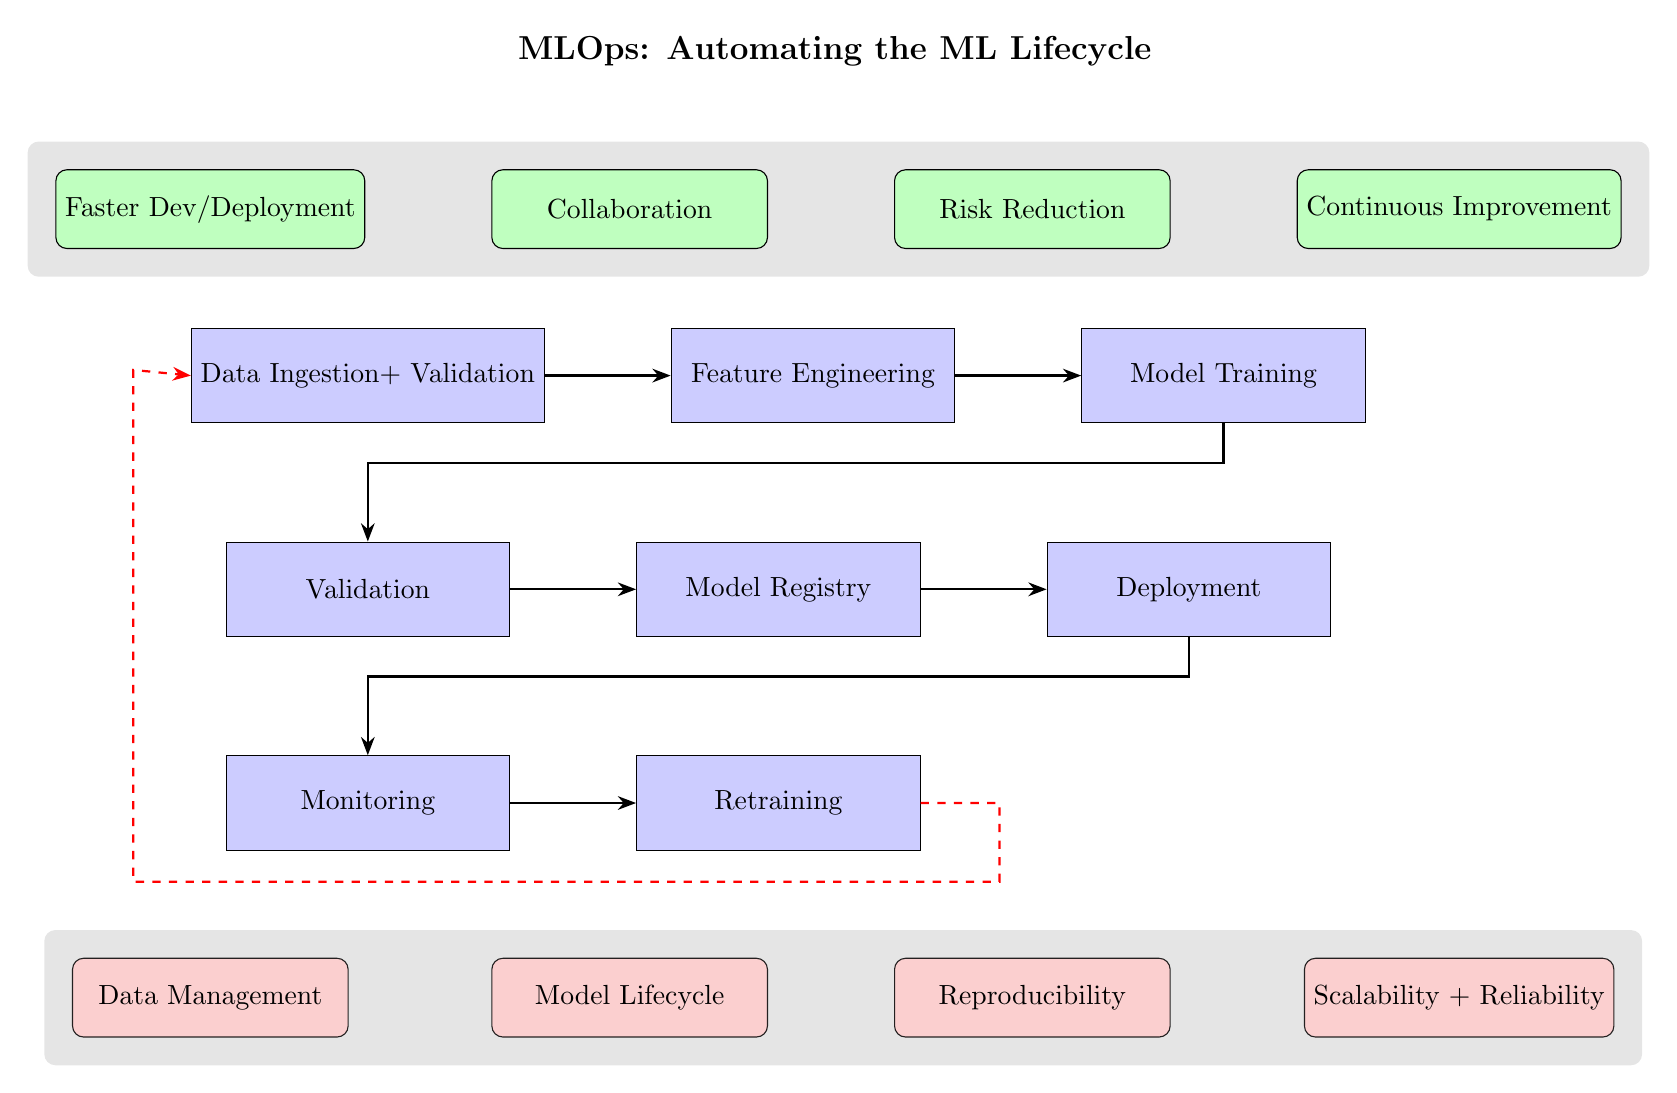
\begin{tikzpicture}[node distance=1.4cm and 1.6cm]

% Top Layer: Goals
\node (g1) [goal] {Faster Dev/Deployment};
\node (g2) [goal, right=of g1] {Collaboration};
\node (g3) [goal, right=of g2] {Risk Reduction};
\node (g4) [goal, right=of g3] {Continuous Improvement};

% Bounding box around the top row
\begin{scope}[on background layer]
  \node[fill=gray!20, rounded corners, fit=(g1)(g4), inner sep=10pt] {};
\end{scope}

% Middle Layer: Pipeline (grouped into three horizontal boxes per row)
\node (data) [component, below=1cm of g1, xshift=2cm] {Data Ingestion \\ + Validation};
\node (features) [component, right=of data] {Feature Engineering};
\node (training) [component, right=of features] {Model Training};

\node (validation) [component, below=1.5cm of data] {Validation};
\node (registry) [component, right=of validation] {Model Registry};
\node (deploy) [component, right=of registry] {Deployment};

\node (monitor) [component, below=1.5cm of validation] {Monitoring};
\node (retrain) [component, right=of monitor] {Retraining};

% Arrows in pipeline
\draw [arrow] (data) -- (features);
\draw [arrow] (features) -- (training);
\draw [arrow] (training.south) -- ++(0,-0.5) -| ($(validation.north)+(0,0.5)$) -- (validation.north);
\draw [arrow] (validation) -- (registry);
\draw [arrow] (registry) -- (deploy);
\draw [arrow] (deploy.south) -- ++(0,-0.5) -| ($(monitor.north)+(0,0.5)$) -- (monitor.north);
\draw [arrow] (monitor) -- (retrain);

% Bottom Layer: Challenges
\node (c1) [challenge, below=9cm of g1] {Data Management};
\node (c2) [challenge, below=9cm of g2] {Model Lifecycle};
\node (c3) [challenge, below=9cm of g3] {Reproducibility};
\node (c4) [challenge, below=9cm of g4] {Scalability + Reliability};

% Bounding box around the bottom row
\begin{scope}[on background layer]
  \node[fill=gray!20, rounded corners, fit=(c1)(c4), inner sep=10pt] {};
\end{scope}

% Feedback loop with clearer path
\coordinate (loopa) at ($(retrain.east)+(1.0,0)$);
\coordinate (loopb) at ($(loopa)+(0,-1.0)$);
\coordinate (loopc) at ($(loopa)+(-11,-1.0)$);
\coordinate (loopd) at ($(loopc)+(0,6.5)$);

\draw[arrow, dashed, red] (retrain.east) -- (loopa)
  -- (loopb) -- (loopc)
  -- (loopd) -- (data.west);

% Title
\node at ($(g1)!0.5!(g4) + (0,2)$) [font=\bfseries\large] {MLOps: Automating the ML Lifecycle};

\end{tikzpicture}

\end{document}
